\documentclass{chi2011}
\usepackage[pdftex]{hyperref}
\usepackage[backend=bibtex,style=verbose-trad2]{biblatex}
\usepackage{enumitem}
\usepackage{scrextend}
\usepackage{graphicx}
\hypersetup{%
pdftitle={Your Title},
pdfauthor={Your Authors},
pdfkeywords={your keywords},
bookmarksnumbered,
pdfstartview={FitH},
colorlinks,
citecolor=black,
filecolor=black,
linkcolor=black,
urlcolor=black,
breaklinks=true,
}

\pagenumbering{arabic}  % Arabic page numbers for submission.  Remove this line to eliminate page numbers for the camera ready copy

\bibliography{final_report}
\begin{document}
% To make various LaTeX processors do the right thing with page size.
\special{papersize=8.5in,11in}
\setlength{\paperheight}{11in}
\setlength{\paperwidth}{8.5in}
\setlength{\pdfpageheight}{\paperheight}
\setlength{\pdfpagewidth}{\paperwidth}

% Use this command to override the default ACM copyright statement
% (e.g. for preprints). Remove for camera ready copy.
% \toappear{Submitted for review to CHI 2011.}

\title{CMPT481 Project Report}
\numberofauthors{3}
\author{
\alignauthor Peggy Anderson\\
    \email{peggy.anderson@usask.ca}
    \alignauthor Chris Penner\\
    \email{clp848@mail.usask.ca}
    \alignauthor Jonathan Baxter\\
    \email{jab231@mail.usask.ca}
}

\maketitle

\section{Problem and Motivation}

In 1980, the ratio for debt-to-income in Canada was 66\%; that ratio passed
150\% in 2011. 
\autocite[1]{STATSCAN:1}
At a young age many Canadians are
taught how to count and spend money; however not all are taught how to budget
effectively. Whether you are a business owner, student, or bringing home the
bacon for your family; it is important to budget. Budgeting allows a person to
determine if they will have enough money for their needs and allows them to
plan for the things they want. The reason people fall in to debt is that they
are spending more than they expected to spend. If a person was to plan ahead
and set aside a predetermined amount of money for each week or month and could
visualize their spending habits it would allow them to better prioritize their
budget and find areas to increase savings.

It can be easy to forget to add expenses as they occur throughout the day.
Some reasons for this are that the method of inputting their expenses may be
too time-consuming or difficult to use; or that their budgeting application is
not available on their mobile device. Many of the current applications that
are purposed towards tracking weekly or monthly recreational budgets (non
re-occurring bills and expenses) are not easy to use or engaging for the user.
Visualization techniques present in other applications tend to focus solely
on the amount of money spent in each category, however this overlooks the
primary purpose of budgeting and does not deliver the information of how the
amount spent relates to the user's savings goals. Many applications sacrifice
ease-of-use by adding clutter for additional (often unused) features. When
navigating many of these applications it can seem like there is ”too much
going on”. Accessibility of the application can also be an issue, disparity
in the interface between the Desktop and mobile versions can be a confusing
experience. Some applications are not available on all devices.

\section{Related Literature and Background}
\section{Description of The System}

    \subsection{Initial Prototype}

    The intention was to build an application that was as easy to use as
    possible, users should be able to jump right into the tasks without prior
    training and be able to complete them confidently and successfully. The
    easiest way to accomplish this was to minify the scope of the application
    to its simplest possible subset. Minimizing the number of actions available
    simplifies the interface and allows the user to navigate confidently.

    In the initial "Wizard of Oz" style paper prototype the interface was pared
    down to only 3 screens, one for each of the tasks users are allowed to
    perform:

    \begin{itemize}[noitemsep]
        \item Add an expense
        \item View expenses
        \item Customize budget allowances
    \end{itemize}

    As with any design process it was quickly discovered during trials that
    it was unclear how to perform certain actions; for instance there was no
    functionality for cancelling or removing an expense. Each hiccup was noted
    and changes were prioritized for the next prototyping stage.

    \subsection{Adjustments}
    
    The next prototype was constructed as a fully interactive and functional
    web application using Javascript, html and CSS. This allowed us to
    implement the functionality which was missing from our paper prototypes
    such as animations, calculations, and the use of real data.

    A critical analysis was performed on the data collected from the
    paper-prototype trials. This inspired a focus on displaying the information
    available as clearly as possible. Naturally the implementation met some
    obstacles and decisions were made to cut or work around some features.
    Features which were cut or altered include:

    \begin{itemize}[noitemsep]
        \item Saving data across sessions
        \item Cancelling expenses
        \item Viewing individual expenses
        \item Cancel buttons/back buttons
        \item Adding additional expense categories
    \end{itemize}

    Many features were determined to be "nice to have" but not crucial for the
    testing stage of this level of prototype. These concerns are addressed
    again in the retrospective portion of the report.

    Overall the choice of web technologies suited the implementation well;
    particularly the ability to use the same prototype on mobile and desktop.
    A familiarity with React and Redux allowed quick bug-free edits when
    concerns regarding functionality or layout were raised. The use of Redux
    specifically simplified the problem of syncing data across the application
    trivial. These choices were made within a forward thinking context, if the
    application were to move forward to large scale deployment the code may
    progress towards that goal.

	\begin{figure}[h!]
		\caption{Desktop Interface}
		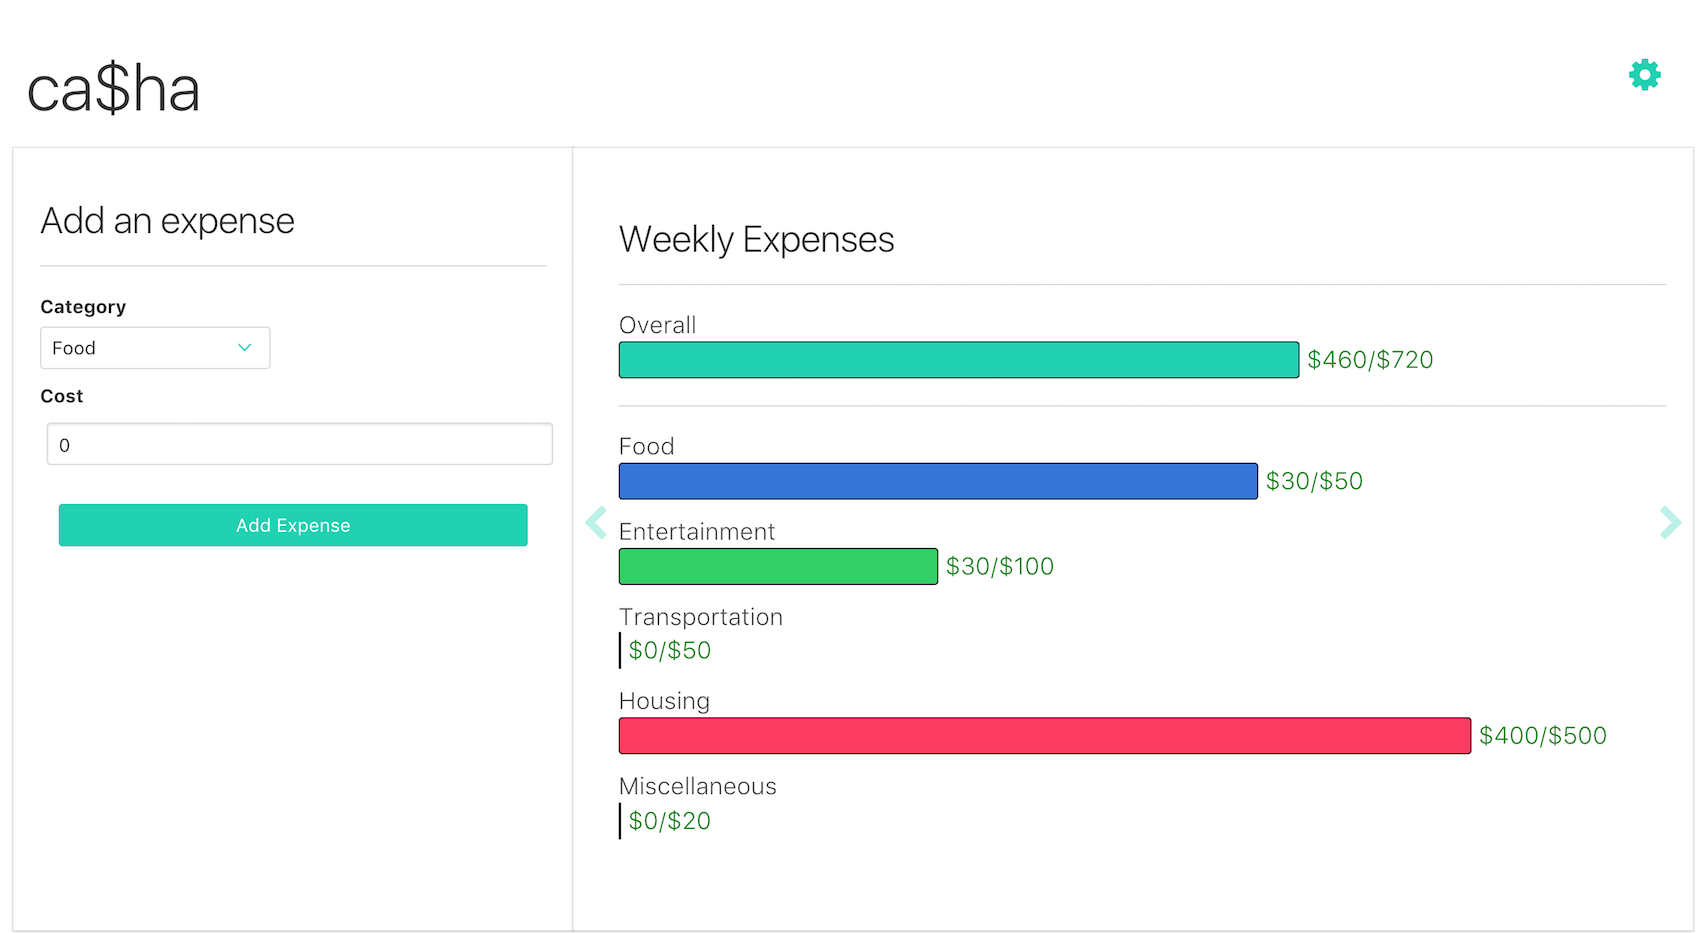
\includegraphics[width=\linewidth]{desktop-main.png}
	\end{figure}

    One of the greatest difficulties was that of creating a responsive
    layout that allowed code re-use across Mobile and Desktop devices. The
    preference was for the interfaces to be similar enough to allow habits
    formed on one device to transfer to the other. To this end CSS media-query
    rules were used extensively alongside the responsive CSS framework
    Bulma.io. Google Chrome's developer tools were instrumental in testing
    the interface on multiple mobile devices.

    Another challenge was the limited screen real-estate on mobile devices.
    Navigation items needed to be accessible without getting in the way.
    Additional complexity was added to the application to hide and show certain
    screens since there is not enough room on a mobile device for all screens
    to be showing at the same time.

	\begin{figure}[h!]
		\caption{mobile Interface}
		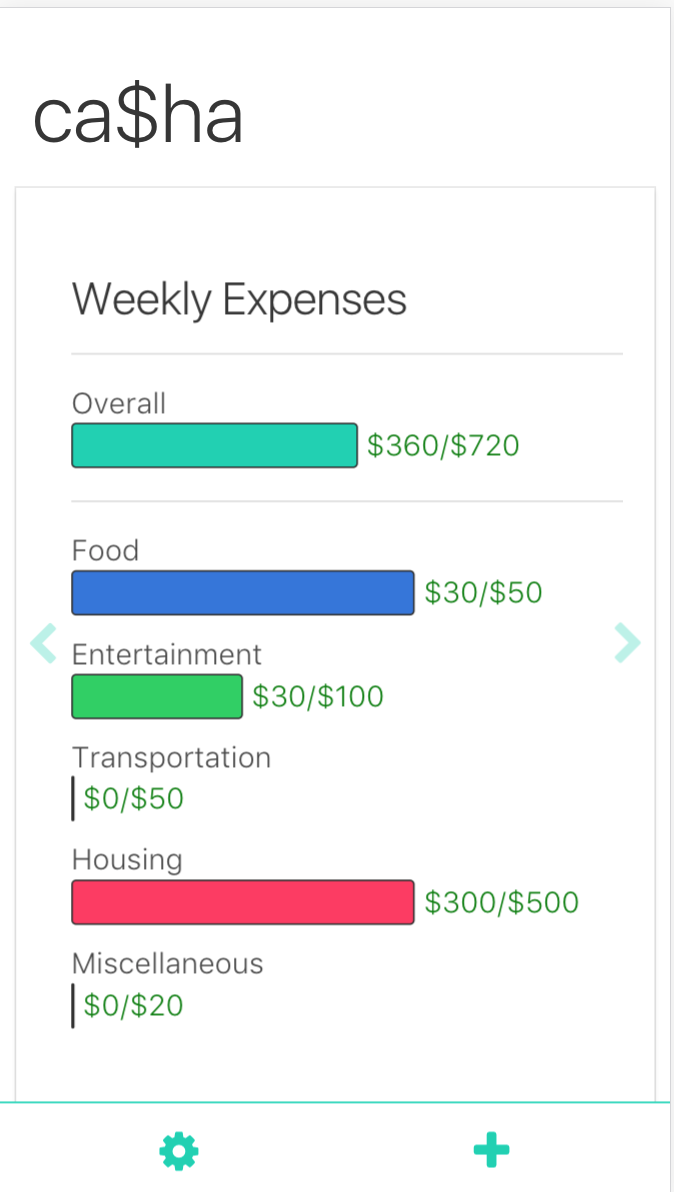
\includegraphics[scale=0.5]{mobile-charts.png}
	\end{figure}

    \subsection{Retrospective}

    As expected, user testing of the interactive prototype revealed yet more
    flaws, but also successes in the design.

    The application failed to account for the change in idioms between mobile
    and desktop; for instance users tried to edit categories or add expenses
    by touching interface elements. Most users mentioned that they would like
    more functionality, many of the requested features were originally part our
    the design but were left out due to time constraints, cluttering of the
    interface, or implementation difficulties.

    It seemed that the most difficulty encountered by users was found in
    navigating between features and the discoverability of functionality. This
    suggests that this is an area of potentially large benefit with lower
    amounts of work.

    Some requested features were deliberately left out. One user mentioned that
    they prefer that their budgeting app links to their bank account and tracks
    their expenses automatically, this pedigree of feature was not only this
    out of scope for the time-frame of the project, but it is also contrary
    to the design principles of being as simple as possible. Several other
    features would be rejected for the purposes of keeping the interface clean
    and simple.

\section{Evaluation with User Reports}

	\subsection{Goals, Approach and Rational for the Evaluation}

		\subsubsection{Goals}

		The primary goal of our project is for users to use our application to continuously track their
		expenses. It is our belief that if the application is easy to use through an intuitive
		interface and navigation then the user will also be able to input expenses quickly and efficiently.
		If the user can quickly tell us how much they have spent in a specific category after expenses have
		been entered then it confirms that the application is presenting a clear visualization of the data.
		Unfortunately the continued use of the application can not be tested within the scope of this class
		since that would require multiple interviews with the test users to evaluate their usage and a
		high-fidelity prototype.

		\subsubsection{Approach and Rational for the Evaluation}

        Interviews were employed to evaluate our goals. The questions were designed
        to determine what users require to make their budgeting experience with the
        application the most enjoyable.


	\subsection{Actual Participant Pool and Other Execution Details}

	A mixture of family and friends represented the users for the test cases that follow.

	\begin{labeling}{Users}
		\item [User 1] An individual who has limited experience with computers.  
		\item [User 2] An individual who has a degree in computer science and may offer some valuable criticisms. 
		\item [User 3] Older demographic who has budgeted using other methods in the past.
		\item [User 4] A business student who has studied budgeting.
	\end{labeling}


	\subsection{Divergence from Milestone III Evaluation Plan}

 Upon implementing the Medium Fidelity-Prototype the task list had diverged
 from what the original scope of functionality had been. Instead of only three
 tasks, the application could now perform five different tasks:
	
	\begin{itemize}[noitemsep]
		\item Add an expense (unchanged)
		\item View expenses over a weeks/months/years time (unchanged)
		\item Change an overall budget (unchanged)
		\item Change a category name
		\item Set a budget limit for one or all categories
	\end{itemize}

        It had originally been planned that the redesign would offer cancellation
        of actions (forms etc.) to improve the user experience, however due to
        implementation difficulties this feature was not included.

	\subsection{Results}

	While examining the results from the interviews it was clear that there were both positive and 
	negative themes. The users appeared to have a preconceived notion of how the application should
	work from applications they had used in the past, even from apps unrelated to budgeting. Due to this
	(unintentional) knowledge transfer many users were confused for reasons we had not anticipated.
	
	Some common themes amongst the users were:
	\begin{itemize}[noitemsep]
		\item Enjoyed Similar interfaces between mobile and desktop
		\item It was easy and quick to add expenses
		\item The animations were pleasing
	\end{itemize}

        The similarity between the desktop and mobile versions of the application
        allowed users to switch between the two with minimal confusion once they had
        learned how to use the application. The animations engaged the users when they
        had added expenses into the application, one user was surprised and said "Oh!
        Fancy."

        Some users requested additional features:
	\begin{itemize}[noitemsep]
		\item Additional customization
		\begin{itemize}[noitemsep]
			\item Ability to pick default view
			\item Ability to add more categories
		\end{itemize}
		\item More in-depth data 
		\item Ability to click a category's label or the bar to edit the name of the category or view more data. 
		\item Cancel Buttons
	\end{itemize}
	
    The users wanted to be able to change the default view of budgeting data so
    they could choose which charts were visible (from weekly/monthly/yearly).
    Some also wanted the option to be able to see a record of individual
    expenses as their primary view. These requests show the general theme
    that that users wanted more data about their habits to be available to
    them; e.g. a breakdown of each individual expense, the amount they spent,
    and when and where they spent it. Most users intuitively thought that
    additional data could be accessed by clicking on the category name/chart (though the feature had not been
    implemented).

    Confusion occured in regards to the charts because many users were unsure
    as to the scale of the chart (when no budget limit for a category was set
    the default was \$100). Users wanted an indicator that they were 
    close to their budget limit. 

    There were some idiosyncracies of the prototype that caused confusion as
    well. Due to the way the prototype was implemented, refreshing the page or
    clicking the "back" button on the browser would erase any expenses that
    had been entered. This of course was simply a limitation of the current
    phase of prototype. The fact that the application was simply a website also
    caused difficulty when one user cried out in frustration as they hit their
    phone's back button to return to the previous page, but instead closed the
    application entirely.
        
    User \#2 mentioned some design ideas; suggesting to create a widget for mobile
    devices and to provide customization options through the widget. Perhaps the
    user could see total amount spent from the budget, see the total remaining
    amount from the budget, or some combination of the above.
        
    User \#4 suggested that making the "Add Expense" page the default screen would
    make adding expenses even quicker.
        
    It was observed by all users that the cost totals on the charts became
    cut off as their expenses neared their budget amount. There was a strong
    usability concern that the textbox for customizing budget amounts on the
    settings page was too small on mobile devices.

	\subsection{Conclusion}

    The overall opinion of the interface was quite positive and it met the
    initial goals well. The layout of the interface was effective, it was easy
    to use and users had very little trouble performing the provided tasks. As
    before mentioned, the most pervasive theme was that users wanted to be able
    to do more with the application; such as adding more categories and to be
    able to more closely track their spending. In this regard the application
    could still use some improvement. 
    
    Though it was not feasible to test whether users continued to use the
    application over time, the majority of testers said that given a fully
    functional version they would use it regularly. As for the primary goal of
    having a simple and quick to use interface it is clear that the application
    was a success. The testing showed that users could quickly add expenses and
    that they found the charts easy to read.

\section{Final Recommendations}
	
The application could still stand to gain a lot in the way of usability from
some minor tweaks however the chosen approach was valid. The tweaks would
include augmenting the interface to make it more complete. This would allow for
more customizability and a better break down of the spending as was requested
by the users. The settings icon would also be changed since this confused some of the
users. The addition of labels to the icons would solve this confusion.

\subsection{Reflection on Design Process}

Originally the plan was to implement a very simple and slimmed down design
for a budgeting application the biggest observation since that initial plan
is that users wanted more functionality then they actually need. The simple
interface let them easily track basic expenses and fulfilled all the basic
needs of simple budgeting, however users requested many "nice to have" features
which did not contribute directly to this goal.

The overall design of our application changed because of the users. The analysis
of the evaluations of the low-fidelity prototype resulted in a reorganization of the
application layout. Many buttons on the interface were moved. One button
was found to be redundant and was removed. Within the medium fidelity
prototype there were many potential changes to allow users more
customizability.

We learned a lot about the user-centered design process over the course of
the project. The process allowed using feedback to improve the interface
and it is a process that would be beneficial for future projects. It was
decided in hindsight that there are a few things that should have been done
differently. The first being that more time should have been spent on refining
the low-fidelity prototype and that it should have been more interactive. Some
of the issues that appeared in the medium fidelity prototype, such as the
setting button, could have been discovered in the low-fidelity prototype. Using a
different prototyping tool for the low-fidelity prototype may have also made it
easier to find these issues.

The chosen approach for evaluating the prototype worked well and gave enough
information to judge the interface. The semi structured interviews provided
lots of information on different aspects and relayed the reactions users
had to the product. Some issues were discovered by observing the users
interacting with the interface, a couple of them wanted to touch the chart
to add an expense to a category. Using a questionnaire or some other less
expressive medium an issue like this would likely not be discovered. Using a
semi-structured interview was effective.

In this course we learned a lot of useful skills for developing a user
interface. One of the skills that is most useful is how to plan and test an
interface before implementation. Building and iterating on the low-fidelity
prototypes is a cost effective way to test effectiveness before further
investment. In a personal project this would save a lot of time, in a
commercial project this would save a lot of money. Planning the interface is
a skill that will transfer well into future careers. Learning to interview
and get feedback from users was another useful skill. The ability to extract
information from a user is very important, and will apply in the workplace
when requesting feedback or obtaining requirements for a project. There are
many lessons from this project that could be applied to future projects and
interface designs. 

\newpage
\section{Appendices}

	\subsection{A1 - Evaluation Instrument}
	\subsubsection{Tasks Performed by Users}
	\begin{itemize}[noitemsep]
		\item Add different expenses to three different categories
		\item After adding expenses, go to the data visualization screen
		\item Change the name of a category
		\item Change the overall budget limit from its default
		\item Change one category limit
		\item Add more expenses to that category to go over the budget limit
	\end{itemize}
		
	\subsubsection{Pre-Demo}
	\begin{itemize}[noitemsep]
		\item Do you currently or have you ever budget(ed)?
		\begin{itemize}[noitemsep]
			\item (Yes - Probing Question) What method do you use?
			\item (No - Probing Question) Is there a specific reason why?
		\end{itemize}
	\end{itemize}
	
	\subsubsection{Post Desktop Demo}
	\begin{itemize}[noitemsep]
		\item Was there anything that you found to be counter-intuitive?
		\item If you could change/add anything about the app, what would it be? (From desktop perspective)
	\end{itemize}

	\subsubsection{Post Mobile Demo}
	\begin{itemize}[noitemsep]
		\item Was there anything that you found counter-intuitive?
		\item If you could change/add anything about the app, what would it be? (From mobile perspective)
	\end{itemize}


	\subsubsection{Post-Demos}
	\begin{itemize}[noitemsep]
		\item Compare and contrast the mobile interface and the desktop interface.
		\begin{itemize}[noitemsep]
			\item (Probing Question) Which was easiest to use?
			\item (Probing Question) Which made the data more visually clear for you?
		\end{itemize}	
	\item  Compare and contrast this budgeting application with others you've used.
		\begin{itemize}[noitemsep]
			\item (Yes - Probing Question) Which app allowed faster input?
			\item (Yes - Probing Question) Which app allowed more accurate input?
			\item (Yes - Probing Question) Are you more likely to continue using this application or a different one?
			\item (No - Probing Question) Why?
		\end{itemize}
	\item (If they had not budgeted before) If this application were available to you, would you be likely to continue using it? 
	\end{itemize}
	
	
	\subsection{A2 - Raw Data}
	
	\subsection{User \#1}

	\subsubsection{Pre-Demos}
	\begin{itemize}[noitemsep]
		\item Do you currently or have you ever budget(ed)?
		\begin{itemize}[noitemsep]
			\item 
				Yes, using pen and paper.
		\end{itemize}
	\end{itemize}
	
	\subsubsection{Desktop Demo}
	\begin{itemize}[noitemsep] 
		\item Add three expenses to three different categories
		\begin{itemize}[noitemsep]
				\item Tried to click on the expenses graph to add an expense
				\item Made an error adding an expense to the housing category,
					accidentally added it to the food category
		\end{itemize}
		\item changing the name of a category
			\begin{itemize}[noitemsep]
				\item Did not recognize the settings button
				\item Found it easy to add the new category name
				\item Wanted to add a new category not change the name
            \end{itemize}
	\end{itemize}
	
	\subsubsection{Post Desktop Demo}
	\begin{itemize}[noitemsep]
		\item Was there anything thing that you found counter-intuitive?
		\begin{itemize}[noitemsep]
				\item found the setting button confusing, a label would be
					helpful
		\end{itemize}
		\item If you could change/add anything about the app, what would it be? (From desktop perspective)
		\begin{itemize}[noitemsep]
				\item Some way of correcting an amount if input incorrectly
					would be good
		\end{itemize}
	\end{itemize}
	
	
	\subsubsection{Mobile Demo}
	\begin{itemize}[noitemsep] 
		\item Add two expenses to two different categories
		\begin{itemize}[noitemsep]
				\item Took some time to find the plus button
		\end{itemize}
	\item Asked to go to yearly expenses view
	\end{itemize}

	\subsubsection{Post Mobile Demo}
	\begin{itemize}[noitemsep]
		\item Was there anything thing that you found counter-intuitive?
		\begin{itemize}[noitemsep]
			\item No, found the cross over from the desktop made it easy to use
			\item Wished there was more touch interaction on the mobile version
		\end{itemize}
		\item If you could change/add anything about the app, what would it be? (From mobile perspective)
		\begin{itemize}[noitemsep]
				\item I would change the same things as with the Desktop version
		\end{itemize}
	\end{itemize}


	\subsubsection{Post-Demos}
	\begin{itemize}[noitemsep]
		\item Compare and contrast the mobile interface and the desktop interface.
		\begin{itemize}[noitemsep]
			\item It was nice that they both had the same features available
			\begin{itemize}[noitemsep]
				\item (Probing Question) Which was easiest to use?
				\item Mobile was the easiest to use more used to that
						platform
			\end{itemize}
		\end{itemize}	
	\item Compare and contrast this budgeting application with others you've used.
		\begin{itemize}[noitemsep]
				\item Never used a computer for budgeting before but found this
					easy to use
		\end {itemize}
	\item (Probing Question) Are you more likely to continue using this application or a different one?
		\begin{itemize}[noitemsep]
				\item Yes I would continue to use the application since it is
					easier and neater then using paper and pen
		\end{itemize}
	\end{itemize}


	\subsection{User \#2}

	\subsubsection{Pre-Demos}
	\begin{itemize}[noitemsep]
		\item Do you currently or have you ever budget(ed)?
		\begin{itemize}[noitemsep]
			\item 
				Yes. Right now User \#2 doesn't budget actively but they do use Mint.com to make sure old
				accounts don't have stuff on them and go through current accounts to ensure there are no
				unknown purchases. 
				
				In the past they used spreadsheets for projecting, and sometimes User \#2 still uses this
				method for their savings and for bigger purchases. 
				
				User \#2 says that they have a facade for budgeting. "Mint.com sucks for things that run over
				multiple months."
		\end{itemize}
	\end{itemize}
	
	\subsubsection{Desktop Demo}
	\begin{itemize}[noitemsep] 
		\item Add three expenses to three different categories
		\begin{itemize}[noitemsep]
			\item Saw animations and said "Aw thats fancy"
			\item Didn't use the arrows to increment/decrement
			\item Added negative numbers
			\item Found out he could input 'e' (didn't do anything except clear any numbers previously 
			typed) When asked why the letter User \#2 answered "only because I was allowed to"
		\end{itemize}
		\item Go to monthly view
		\begin{itemize}[noitemsep]
			\item Highlighted "Weekly View"
			\item Went into Settings then hit browser back button and that caused the application to close
		\end{itemize}
		\item Change the overall budget
		\begin{itemize}[noitemsep]
			\item Tried to add -0.10, changed to "NaN"
		\end{itemize}
		\item Max a category
		\begin{itemize}[noitemsep]
			\item Entered 9.99 then entered 0.01 and it didn't max the category
		\end{itemize}
	\end{itemize}
	
	\subsubsection{Post Desktop Demo}
	\begin{itemize}[noitemsep]
		\item Was there anything thing that you found counter-intuitive?
		\begin{itemize}[noitemsep]
			\item Switching between views, the arrows on side made User \#2 thing that it would go to a 
			history. "Although the forward wouldn't make sense for this."
			\item Click category label to change the name
		\end{itemize}
		\item If you could change/add anything about the app, what would it be? (From desktop perspective)
		\begin{itemize}[noitemsep]
			\item Expected a drop down to toggle views
			\item Add back button to settings page (or a cancel button)
			\item Hover over category label to see a button to edit the name
			\item Want to be able to see if you're increasing or decreasing spending of money of if theres a 
			  certain time of the year you're spending more money (VERY IMPORTANT TO USER - Charting
			  over time)
			\item Can't see actual expenses of what you're spending per day on what day
			\item Only tracking expenses and not income
		\end{itemize}
	\end{itemize}
	
	
	\subsubsection{Desktop Demo}
	\begin{itemize}[noitemsep] 
		\item Add two expenses to two different categories
		\begin{itemize}[noitemsep]
			\item Used "Add Another"
		\end{itemize}
	\item Asked to go to yearly expenses view
		\begin{itemize}[noitemsep]
			\item Didn't swipe
		\end{itemize}
	\end{itemize}

	\subsubsection{Post Mobile Demo}
	\begin{itemize}[noitemsep]
		\item Was there anything thing that you found counter-intuitive?
		\begin{itemize}[noitemsep]
			\item No, but there were things I'd change
		\end{itemize}
		\item If you could change/add anything about the app, what would it be? (From mobile perspective)
		\begin{itemize}[noitemsep]
			\item On Add Expense Page
			\item Make it so the category budget is visible
			\item Add back or cancel button
			\item Light colours for buttons don't look like it's disabled
			\begin{itemize}[noitemsep]
				\item Make it grey, or have a notification to say why you can't add an expense
				\item Can't do anything if there is no category selected, but can do something if there
				  is no expense inputted, weird
			\end{itemize}
			\item In settings 
			\begin{itemize}[noitemsep]
				\item Add back or cancel button
			\end{itemize}
			\item On main page
			\begin{itemize}[noitemsep]
				\item Change arrows to three dots to know to swipe
			\end{itemize}
			\item 
				It would be cool to have a widget so you can add an expense really easily without having 
				to open the app. Customizable widgets too, so if you wanted a quick add expense button, 
				or if you wanted to just see where you were budget wise(total amount spent versus 
				remaining budget amount, OR only total spent, OR only remaining budget amount)
		\end{itemize}
	\end{itemize}


	\subsubsection{Post-Demos}
	\begin{itemize}[noitemsep]
		\item Compare and contrast the mobile interface and the desktop interface.
		\begin{itemize}[noitemsep]
			\item It was nice that they both had the same features available. Mint.com disables some
				  features for their mobile application
			\begin{itemize}[noitemsep]
				\item (Probing Question) Which was easiest to use?
				\begin{itemize}[noitemsep]
					\item Desktop was easiest to use because I can use the refresh button to get out of the
						  settings page without having to hit "Save"
				\end{itemize}
			\item (Probing Question) Which made the data more visually clear for you?
				\begin{itemize}[noitemsep]
					\item No difference
				\end{itemize}
			\end{itemize}
		\end{itemize}	
	\item Compare and contrast this budgeting application with others you've used.
		\begin{itemize}[noitemsep]
			\item It's not a fair comparison because mint.com is a professional product made by an 
				  international finance company
			\item Your app is easier to use if you are not wanting to have it tied to bank accounts, and is
				  easier to add expenses.
			\item I like Mint.com because it has the ability to track not just the value of what you spent
				  but also when and what the expense was for
		\end {itemize}
	\item (Probing Question) What app allowed you faster input?
		\begin{itemize}[noitemsep]
			\item For cash expenses your app is faster, or for expenses if you can't link an account
			\item Mint.com credit card expenses are delayed, however debit transactions are faster
		\end{itemize}
	\item (Probing Question) What app allowed more accurate input?
		\begin{itemize}[noitemsep]
			\item It's the same,  both can still see wha tthe amount is before it gets used
			\item For choosing categories your app is harder, Mint doesn't require me to worry about a
				  box (for inputting the amount)
		\end{itemize}
	\item (Probing Question) Are you more likely to continue using this application or a different one?
		\begin{itemize}[noitemsep]
			\item It has potential, but I wouldn't currently use it.

				  If I were to use it I would want to include location and date of the expense. US is 
				  okay as is, not ideal. I want to be able to go back and change past expenses. I want
				  more data out of the program. Don't want expenses to be summed up. Want monthly budget
				  or yearly budget, don't care about weekly budget. In fact, I want monthly budget to be 
				  the default view, and it not be a sum of the weekly budget. Also the ability to add 
				  income and assets, or my specific bank accounts. 
			\begin{itemize}[noitemsep]
				\item (Probing Question) With those changes would you use this app over Mint.com 
					  consistently? 
				\begin{itemize}[noitemsep]
					\item With those changes? Yes.
				\end{itemize}
			\end{itemize}
		\end{itemize}
	\end{itemize}
	
	
	\subsection{User \#3}
	\subsubsection{Pre-Demos}
	\begin{itemize}[noitemsep]
		\item Do you currently or have you ever budget(ed)?
		\begin{itemize}[noitemsep]
			\item I sort of budget, I write down and calculate my spending on
				paper to track it. 
		\end{itemize}
	\end{itemize}
	
	\subsubsection{Desktop Demo}
	\begin{itemize}[noitemsep] 
		\item Add three expenses to three different categories
		\item Change the name of a category
	\end{itemize}
	
	\subsubsection{Post Desktop Demo}
	\begin{itemize}[noitemsep]
		\item Was there anything thing that you found counter-intuitive?
		\begin{itemize}[noitemsep]
			\item I do not like that it was weekly, couldn't find the monthly version. Tends to
			 budget on a monthly basis. 
			\item I would like it if you could set the monthly view as default
			\item wished that she would could go to a different page then come back and the
			data would stay(we have no server connected)
		\end{itemize}
		\item If you could change/add anything about the app, what would it be? (From desktop perspective)
		\begin{itemize}[noitemsep]
				\item I would like to customize the colours more and add more
					category
				\item  Would like to see a break down on when and what things were spent on
		\end{itemize}
	\end{itemize}
	
	\subsubsection{Mobile Demo}
	\begin{itemize}[noitemsep] 
		\item Add two expenses to two different categories
		\item Asked to go to yearly expenses view
	\end{itemize}

	\subsubsection{Post Mobile Demo}
	\begin{itemize}[noitemsep]
		\item Was there anything thing that you found counter-intuitive?
			\begin{itemize}[noitemsep]
				\item I don't like have to press the plus compared to the desktop but this is
				  because i had to use the desktop first. 
			  	\item Could of flipped graphs to make them all fit on the screen
			\end{itemize}
		\item If you could change/add anything about the app, what would it be? (From mobile perspective)
		\begin{itemize}[noitemsep]
			\item Make the format similar to the desktop so that the add
				expenses is shown all the time
			\item Some sort of remove button to fix amounts that are added
		\end{itemize}
	\end{itemize}

	\subsubsection{Post-Demos}
	\begin{itemize}[noitemsep]
		\item Compare and contrast the mobile interface and the desktop interface.
		\begin{itemize}[noitemsep]
				\item Once I got used to the mobile interface it was as good as
					the desktop and as easy to use
			\begin{itemize}[noitemsep]
				\item (Probing Question) Which was easiest to use?
				\begin{itemize}[noitemsep]
					\item Found the desktop easier because everything was on one
						page
				\end{itemize}
			\item (Probing Question) Which made the data more visually clear for you?
				\begin{itemize}[noitemsep]
					\item It was easier to see the graphs on the mobile since
						that is all that was on the page
				\end{itemize}
			\end{itemize}
		\end{itemize}

		\item After testing this app, would you be likely to continue using it consistently? 
		\begin{itemize}[noitemsep]
				\item Yes I would continue to use, It is easier to use then with
					pen and paper. I also found it faster to use overall since
					it would always be right there on my phone.
		\end{itemize}
	\end{itemize}
	
	
	\subsection{User \#4}
	\subsubsection{Pre-Demos}
	\begin{itemize}[noitemsep]
		\item Do you currently or have you ever budget(ed)?
		\begin{itemize}[noitemsep]
			\item 
				Personally? No, maybe, techincally yes. Never followed it. User \#4 created a budget for the
				sake a creating a budget. Doesn't believe budgets to be beneficial. Here we talked about
				some pros and cons.
				\begin{itemize}[noitemsep]
					\item "I'm a seasonal worker, would make more sense to budget if I had a consistent 
					      income."
					\begin{itemize}[noitemsep]
						\item "Wouldn't it then make more sense to budget? You know you have this much 
							   money for these many months, budget to make sure you end by breaking even or
							   by ending in a surplus."
					\end{itemize}
				\end{itemize}
			\item 
				User \#4 says their way of budgeting is by asking "do I have enough money for the year?" 
				Where they are "Naturally frugal" they don't make many big purchases and when they do it 
				doesn't make a big difference. 
		\end{itemize}
	\end{itemize}
	
	\subsubsection{Desktop Demo}
	\begin{itemize}[noitemsep] 
		\item Add three expenses to three different categories
		\begin{itemize}[noitemsep]
			\item User \#4 had tried using the arrows to increment the amount he was adding but quickly 
				  changed to the num pad.
			\item Asked for clarification if he was adding an expense for a day/week/month/year 
		\end{itemize}
		\item Change the name of a category
		\begin{itemize}[noitemsep]
			\item Clicked on the category name
			\item Clicked on the drop down for adding expenses to a specific category
			\item Clicked on the settings gear and said "ahh"
		\end{itemize}
	\end{itemize}
	
	\subsubsection{Post Desktop Demo}
	\begin{itemize}[noitemsep]
		\item Was there anything thing that you found counter-intuitive?
		\begin{itemize}[noitemsep]
			\item "Add an expense" text makes him think that he can click on it to add an expense, didn't
					immediately realize it was a title. 
			\item Not immediately drawn to the settings gear, clicked on the category title, then the 
				  category bar, then the category drop down (that you want to add an expense to) to try to
				  change the name of the category first.
			\item Scrolling arrows to increment added expense amount is weird, goes up by one.
		\end{itemize}
		\item If you could change/add anything about the app, what would it be? (From desktop perspective)
		\begin{itemize}[noitemsep]
			\item Have the arrows to increment added expense increment amount by 10
			\item Have category names/bars clickable to change category name/add expense/see total expenses
			\item See the arrows to change between weekly/monthly/yearly be more prominent. Didn't notice 
					that until the interviewer pointed them out. 
			\item Have it be more customizable
			\begin{itemize}[noitemsep]
				\item Wants to be able to have more categories (more than 5)
			\end{itemize}
		\end{itemize}
	\end{itemize}
	
	\subsubsection{Desktop Demo}
	\begin{itemize}[noitemsep] 
		\item Add two expenses to two different categories
		\begin{itemize}[noitemsep]
			\item User \#4 missed the "Add Another" button
			\begin{itemize}[noitemsep]
				\item After he added the second expense the interviewer asked him to add another expense 
					  but this time click that button instead of "Done"
			\end{itemize}
		\end{itemize}
	\item Asked to go to yearly expenses view
		\begin{itemize}[noitemsep]
			\item Swiped immediately
		\end{itemize}
	\end{itemize}

	\subsubsection{Post Mobile Demo}
	\begin{itemize}[noitemsep]
		\item Was there anything thing that you found counter-intuitive?
		\begin{itemize}[noitemsep]
			\item "Add Another" button - wasn't sure it would save first entry
			\item Pressing back button on mobile device ruined data
			\item Clicking save "what if I don't want to save it?"
			\item swiping was intuitive - didn't notice arrows though
		\end{itemize}
		\item If you could change/add anything about the app, what would it be? (From mobile perspective)
		\begin{itemize}[noitemsep]
			\item In settings 
			\begin{itemize}[noitemsep]
				\item Change it so that you can see what you're typing in for a category limit
				\item Have more categories!
			\end{itemize}
			\item On main page
			\begin{itemize}[noitemsep]
				\item Click the category label/bar to add expense
				\item Don't like that you can't see budget numbers on screen 
				\item Add indicator that you're getting close to the budget limit, have a bar, half of what
				  you've spent, half what you have left in budget to spend
				\item See what you're spending day/month
			\end{itemize}
		\end{itemize}
	\end{itemize}

	\subsubsection{Post-Demos}
	\begin{itemize}[noitemsep]
		\item Compare and contrast the mobile interface and the desktop interface.
		\begin{itemize}[noitemsep]
			\item Gear was much better on mobile, had to figure it out still though
			\item Pretty much the same
			\item Desktop has stuff you can do from the main page, mobile has another screen (quick and easy to
				  use)
			\begin{itemize}[noitemsep]
				\item (Probing Question) Which was easiest to use?
				\begin{itemize}[noitemsep]
					\item Both were easy
				\end{itemize}
			\item (Probing Question) Which made the data more visually clear for you?
				\begin{itemize}[noitemsep]
					\item Desktop because on mobile the screen is crammed. Have mobile main screen be add expense and data be a separate page showing all 
						  weekly/monthly/yearly on one page.
				\end{itemize}
			\end{itemize}
		\end{itemize}

		\item (If they had not budgeted before) After testing this app, would you be likely to continue using it consistently? 
		\begin{itemize}[noitemsep]
			\item No. It doesn't do much. Want to view list of individual expenses.
			\item More data, what days you spent, how much you spent, how it changes week to week.
		\end{itemize}
	\end{itemize}

    % \bibliographystyle{acm-sigchi}

\newpage
\printbibliography

\end{document}
